\section{Pile ou face avec \st}

%   logo mb dans la table des matières
\logo{st}

% style de page micro:bit
\pagestyle{st}

\subsection{Description}

\subsubsection{Objectif}

\begin{formule}https://www.overleaf.com/8232568565gwgstdqzhjfk
Le but de ce projet est de simuler une expérience aléatoire de lancer de pièce avec une carte \st. 
\end{formule}


\subsubsection{Intérêt}
Bien évidemment, travailler avec une carte \st n'exclut pas de réaliser des expériences aléatoires réelles (pièces, dés, etc.). Cependant, il est très intéressant pour l'enseignant d'utiliser des \st dans cette partie du programme.
\begin{description}
    \item [Simplicité de la situation.] La situation est très simple à expliquer et les élèves comprennent le but à atteindre. L'absence de difficulté mathématique rend cette situation particulièrement simple à mettre en œuvre.
    \item [Motivation des élèves.] L'envie de programmer un objet connecté est grande pour les élèves. Cette façon de programmer, \emph{utile, concrète et appliquée}, leur correspond parfaitement.
    \item [De nombreuses solutions/améliorations possibles.] Comme pour bien des projets, il y a plusieurs façons d'arriver à la solution. Par ailleurs, les élèves peuvent apporter ou proposer de nombreuses améliorations. La programmation par bloc, exempte de difficulté syntaxique, est particulièrement adaptée à la créativité.
    \item [Travail mathématique sur la modélisation.] Cette compétence n'est pas facile à mettre en œuvre. Ici, l'absence de difficultés mathématiques rend ce travail beaucoup plus accessible à tous.
    \item [Initiation aux différents capteurs] Aux travers cette activité on peut commencer à utiliser l'accéléromètre (en secouant la carte) , le magnétomètre (en approchant un aimant ) etc..

\end{description}


\subsubsection{Matériel}
\begin{itemize}
    \item 1 $\times$ \matosSt \emph{(facultatif car le simulateur peut suffire)}
    \item 1 $\times$ accès internet : IDE programmation par bloc \url{https://makecode.st.com/}
\end{itemize}


\newpage
\subsection{Progression proposée}

\begin{methode}
Voici la progression proposée aux élèves. L'objectif est atteint dès la troisième étape. Les étapes suivantes, de niveau expert, sont du bonus.
\begin{enumerate}
    \item
        \textbf{Initiation - Premier modèle.} \\
        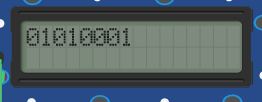
\includegraphics[width=3.5cm]{res/st-pf-00.png}\\Afficher un \texttt{0} ou un \texttt{1} de façon aléatoire. Pour préparer la suite et pour plus de lisibilité, nous proposons dès maintenant de créer et d'utiliser la fonction \texttt{nTirage}.
    \item 
        \textbf{Intermédiaire - Pile ou Face.}\\
        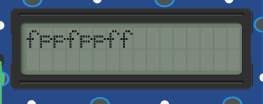
\includegraphics[width=3.5cm]{res/st-pf-01.png}\\Afficher un \texttt{p} ou un \texttt{f} de façon aléatoire.
    \item 
        \textbf{Intermédiaire - 16 tirages.}\\ 
        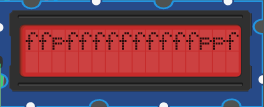
\includegraphics[width=3.5cm]{res/st-pf-02.png}\\Afficher d'un coup 16 tirages aléatoires. Nous donnons à l'élève une nouvelle fonction : \texttt{efface}. Elle permet d'effacer l'écran LCD avant chaque tirage (sinon on voit rien). De plus, le fond d'écran chage de couleur de façon aléatoire (c'est fun!)
    \item
        \textbf{Expert - Initialisation.} \\
        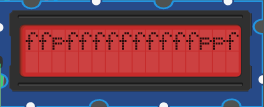
\includegraphics[width=3.5cm]{res/st-pf-02.png}\\Ajouter la fonction \texttt{initialisation} qui lance 10 fois la fonction \texttt{efface} (ce qui fait une petite animation de couleurs). Utiliser cette fonction pour initialiser \st au démarrage et lors d'un appui long sur le bouton.
    \item
        \textbf{Expert - 32 tirages.} \\
        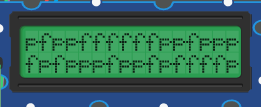
\includegraphics[width=3.5cm]{res/st-pf-04.png}\\Afficher maintenant les tirages sur 2 lignes.
    \item
        \textbf{Expert - Enregistrer les effectifs.} \\
        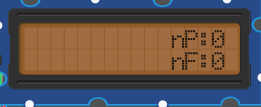
\includegraphics[width=3.5cm]{res/st-pf-05-1.png} \quad
        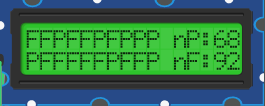
\includegraphics[width=3.5cm]{res/st-pf-05-2.png}\\Création de deux variables \texttt{nP} et \texttt{nF} qui stockent le nombre total de piles et de faces obtenues. Afficher les valeurs de ces variables sur l'écran. Pour cela, effectuer seulement 10 tirages aléatoires par ligne (au lieu de 16) afin de laisser la place pour l'affichage de 5 caractères. 
\end{enumerate}
\end{methode}

%
% activité de niveau 
%
\newpage
\subsection{Niveau initiation - Premier modèle }
\subsubsection{Activité élève}

% commande perso \CARTOUCHE
%   5 paramètres : 
%       * durée
%       * public
%       * travail en maths
%       * travail en sciences
%       * travail en algo
\cartouche{0,5 h}{2de}{expérience aléatoire}{}{affichage ; événement ; fonction}



%
%   ELEVE
%
\begin{wrapfigure}[4]{r}{3cm}
    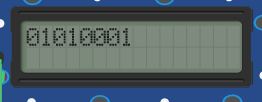
\includegraphics[width=\linewidth]{res/st-pf-00.png}
\end{wrapfigure}

\begin{eleve}    
    \texttt{\textsc{Mission} : utiliser vos \st pour jouer à \emph{Pile ou Face}!}
    
    \begin{description}
        \item [Connectez vous] sur l'interface de programmation de votre \st (\url{https://makecode.st.com/}).
        \item [Utiliser les instructions] ci-dessous pour simuler un jeu de pile ou face.
    \end{description}
    
    \centerline{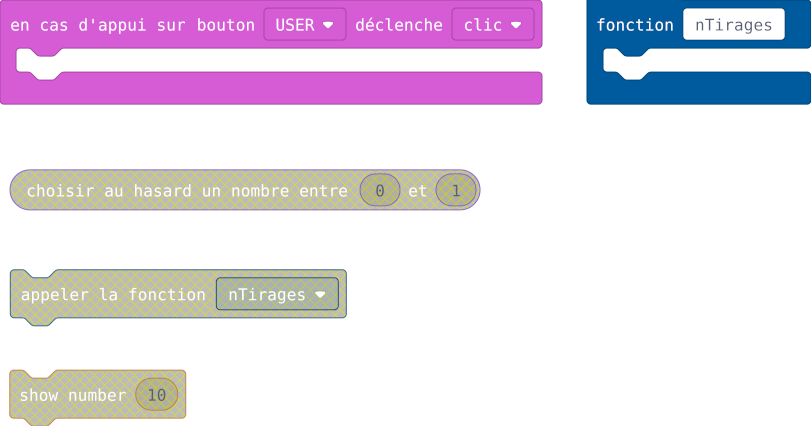
\includegraphics[width=0.75\linewidth]{res/st-pf-00-eleve.png}}
\end{eleve}
%
%   PROF
%

\subsubsection{Notes pour l'enseignant}


\begin{minipage}{0.7\linewidth}
    \begin{methode}~\\
    Proposition de résolution :
    
    \centerline{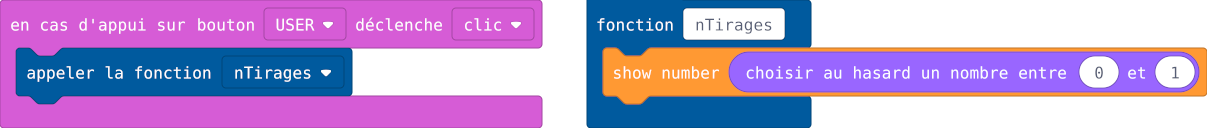
\includegraphics[width=\linewidth]{res/st-pf-00-prof.png}}
    \end{methode}
\end{minipage}
\hfill
\begin{minipage}{0.3\linewidth}
    \begin{remarque}~\\
        La proposition de solution \emph{interactive} est accessible en ligne \url{https://makecode.com/_EMYM0YfT11A6}.
    \end{remarque}
\end{minipage}


%
% activité de niveau 
%
\newpage
\subsection{Niveau intermédiaire - Pile ou Face}
\subsubsection{Activité élève}

% commande perso \CARTOUCHE
%   5 paramètres : 
%       * durée
%       * public
%       * travail en maths
%       * travail en sciences
%       * travail en algo
\cartouche{0,5 h}{2de}{expérience aléatoire}{}{affichage ; événement ; fonction ; condition}



%
%   ELEVE
%
\begin{wrapfigure}[4]{r}{3.5cm}
    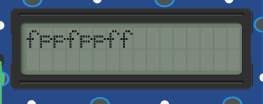
\includegraphics[width=\linewidth]{res/st-pf-01.png}
\end{wrapfigure}
\begin{eleve}
    \texttt{\textsc{Mission} : améliorer votre simulateur}
    
    Utiliser les blocs ci-dessous pour remplacer les \texttt{0} et les \texttt{1} par des \texttt{p} ou \texttt{f}.
   
    \centerline{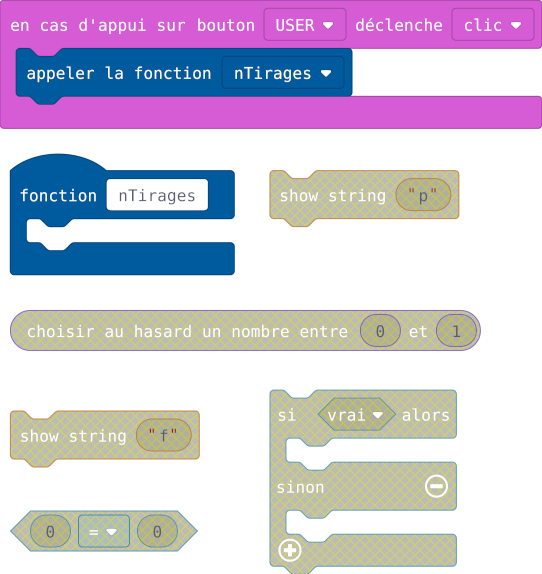
\includegraphics[width=0.65\linewidth]{res/st-pf-01-eleve.png}}
\end{eleve}

\newpage

\subsection{Notes pour l'enseignant}

\begin{minipage}[t]{0.5\linewidth}
    \begin{methode}~\\
        Proposition de résolution :\\
        \centerline{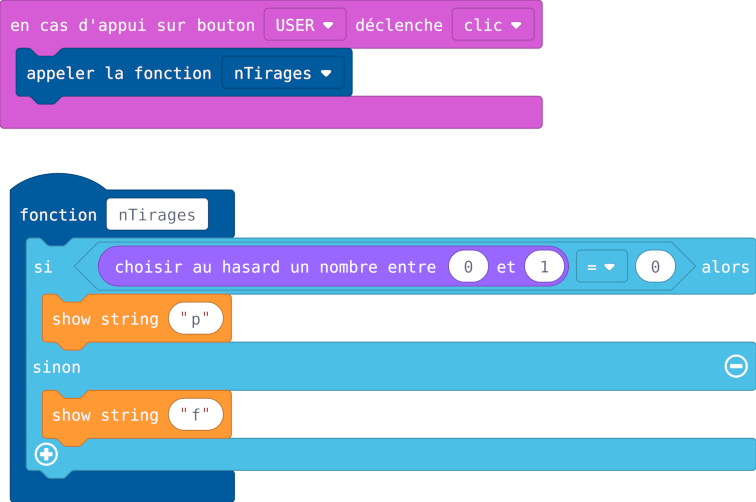
\includegraphics[width=\linewidth]{res/st-pf-01-prof.png}}
    \end{methode}
\end{minipage}
\hfill
\begin{minipage}[t]{0.5\linewidth}
    \begin{remarque}~\\
        La proposition de solution \emph{interactive} est accessible en ligne \url{https://makecode.com/_MysE701XAHpo}.
    \end{remarque}
\end{minipage}

%
% activité de niveau 
%
\newpage
\subsection{Niveau intermédiaire - 16 tirages}
\subsubsection{Activité élève}

% commande perso \CARTOUCHE
%   5 paramètres : 
%       * durée
%       * public
%       * travail en maths
%       * travail en sciences
%       * travail en algo
\cartouche{0,5 h}{2de}{expérience aléatoire}{}{affichage ; événement ; fonction ; condition ; boucle}


%
%   ELEVE
%
\begin{wrapfigure}[4]{r}{3.5cm}
    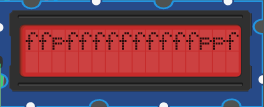
\includegraphics[width=\linewidth]{res/st-pf-02.png}
\end{wrapfigure}

\begin{eleve}    
    \texttt{\textsc{Mission finale} : utiliser la puissance de l'électronique pour effectuer 16 tirages simultanés !}
    
    \begin{minipage}[t]{0.3\linewidth}\raggedright
        En vous aidant des instructions proposées, modifier votre programme pour afficher simultanément \emph{16 tirages sur la première ligne}.
    
        N'oubliez d'ajouter la fonction \texttt{efface} qui permet d'effacer l'écran LCD de votre \st. 
    \end{minipage}
    \hfill
    \begin{minipage}[t]{0.65\linewidth}
        \centering
        \vspace{0pt}
        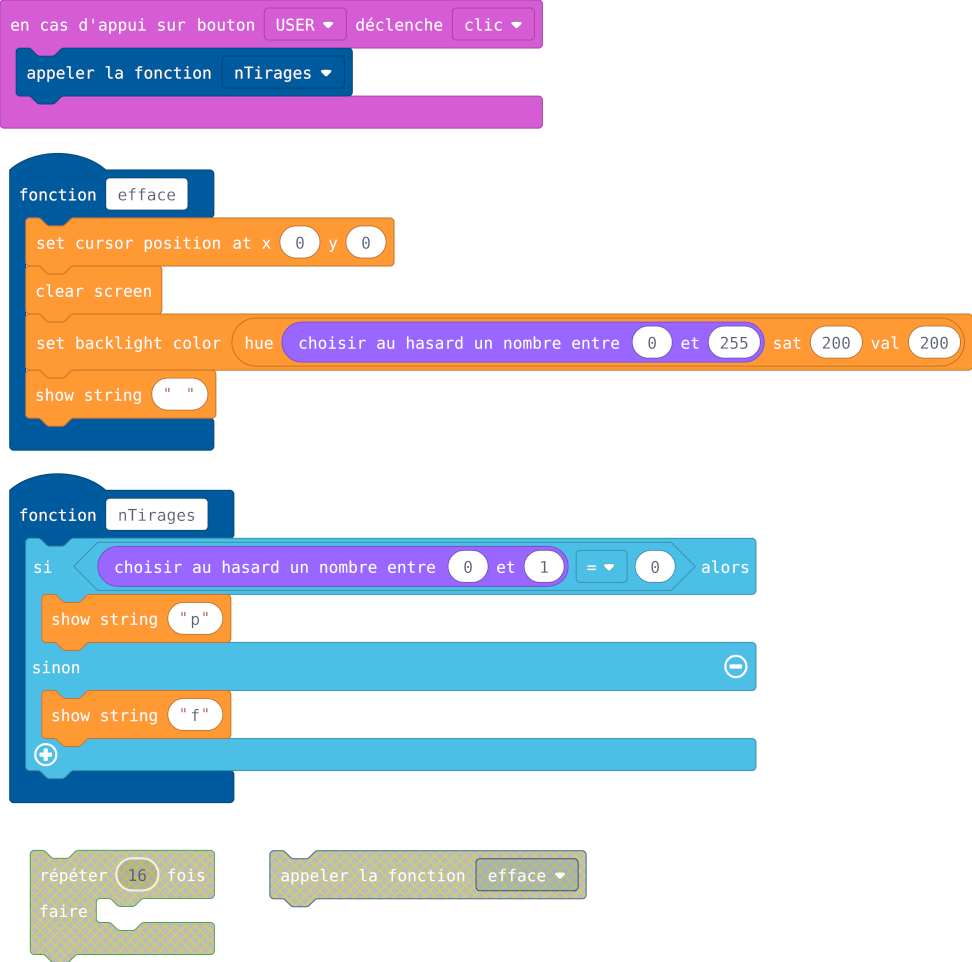
\includegraphics[width=\linewidth]{res/st-pf-02-eleve.png}
    \end{minipage}
\end{eleve}

\newpage

\begin{minipage}[t]{0.8\linewidth}
    \begin{methode}~\\
    Proposition de résolution :
    
    \centerline{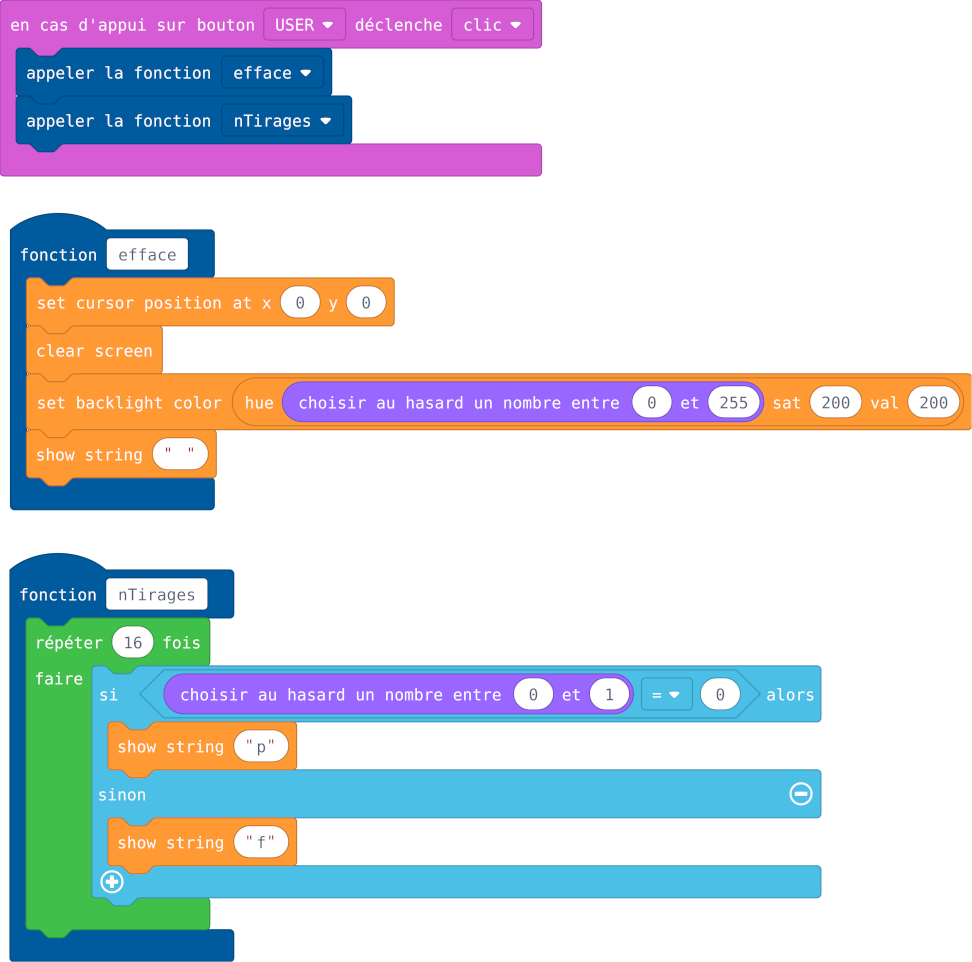
\includegraphics[width=\linewidth]{res/st-pf-02-prof.png}}
    \end{methode}
\end{minipage}
\hfill
\begin{minipage}[t]{0.2\linewidth}
    \begin{remarque}~\\
        La proposition de solution \emph{interactive} est accessible en ligne \url{https://makecode.com/_711WJtAupKRX}.
    \end{remarque}
\end{minipage}
%
% activité de niveau 
%
\newpage
\subsection{Niveau expert - Initialisation}
\subsubsection{Activité élève}

% commande perso \CARTOUCHE
%   5 paramètres : 
%       * durée
%       * public
%       * travail en maths
%       * travail en sciences
%       * travail en algo
\cartouche{0,5 h}{2de}{expérience aléatoire}{}{affichage ; événement ; fonction ; condition ; boucle}


%
%   ELEVE
%
\begin{wrapfigure}[3]{r}{3.5cm}
    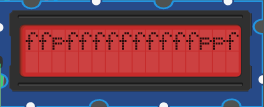
\includegraphics[width=\linewidth]{res/st-pf-02.png}
\end{wrapfigure}

\begin{eleve}    
    \texttt{\textsc{Mission experte 1/3} : initialiser la carte}
    
    
    \begin{minipage}[t]{0.2\linewidth}
        Afin de préparer les améliorations à venir, créez une \emph{nouvelle fonction} \texttt{initialisation}.
        
        Elle doit exécuter 10 fois la fonction \texttt{efface}, ce qui fait très jolie avec l'écran coloré !
        
        Cette fonction \texttt{initialisation} sera appelée au démarrage de votre \st et aussi lors d'un \emph{appui long sur le bouton}.
    \end{minipage}
    \hfill
    \begin{minipage}[t]{0.75\linewidth}
        \vspace{0pt}
        \centerline{
            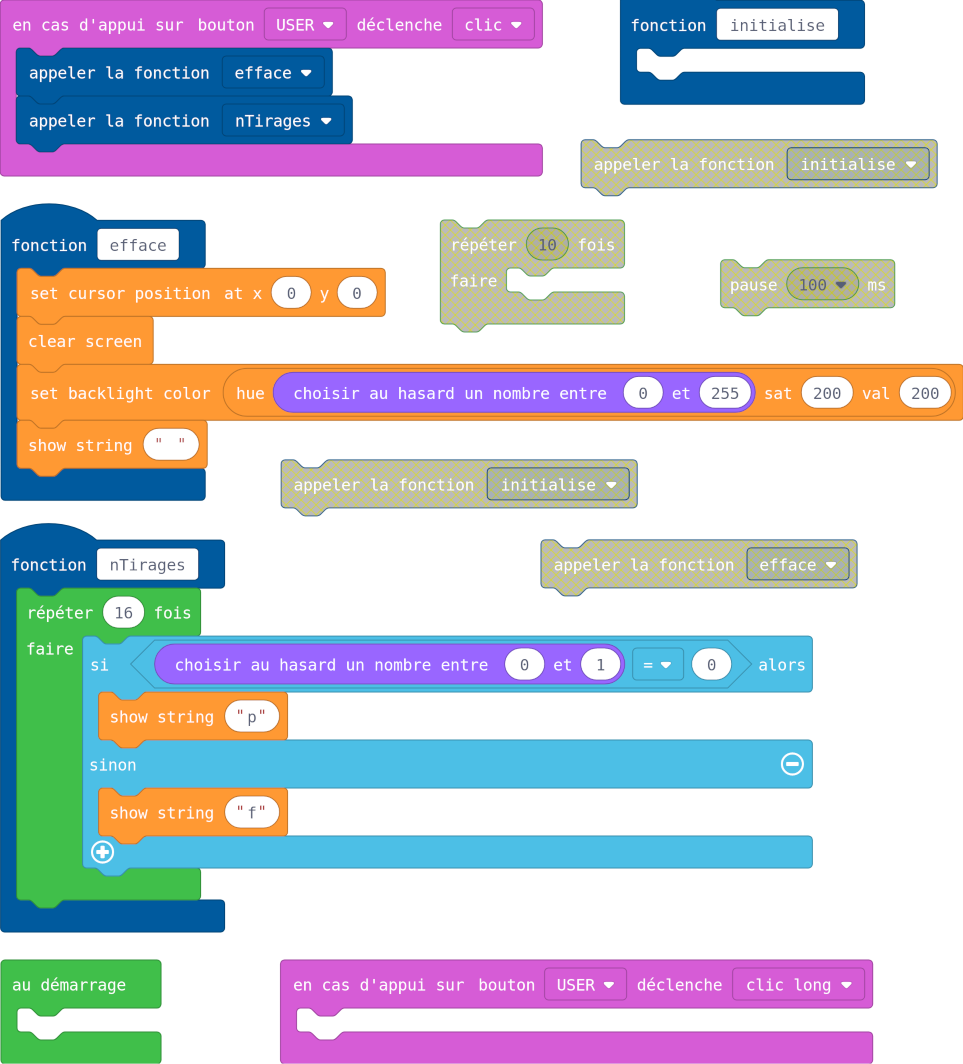
\includegraphics[width=\linewidth]{res/st-pf-03-eleve.png}}
    \end{minipage}
    

\end{eleve}

\newpage

\begin{minipage}[t]{0.8\linewidth}
    \begin{methode}~\\
        Proposition de résolution :
        
        \centerline{
            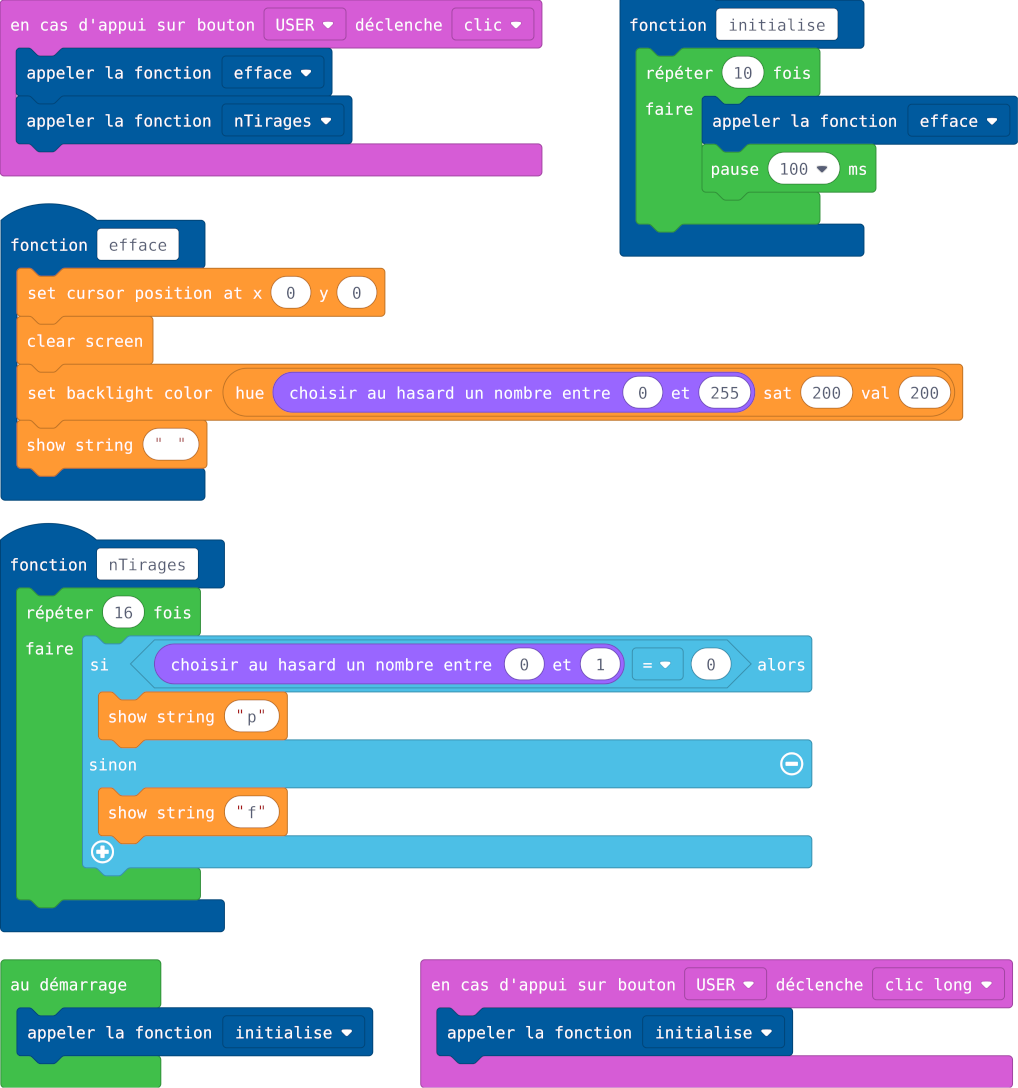
\includegraphics[width=\linewidth]{res/st-pf-03-prof.png}}
    \end{methode}
\end{minipage}
\hfill
\begin{minipage}[t]{0.2\linewidth}
    \begin{remarque}~\\
    La proposition de solution \emph{interactive} est accessible en ligne \url{https://makecode.com/_c3mKWL3fFX6A}.
\end{remarque}
\end{minipage}





%
% activité de niveau 
%
\newpage
\subsection{Niveau expert - 32 tirages}
\subsubsection{Activité élève}

% commande perso \CARTOUCHE
%   5 paramètres : 
%       * durée
%       * public
%       * travail en maths
%       * travail en sciences
%       * travail en algo
\cartouche{0,5 h}{2de}{expérience aléatoire}{}{affichage ; événement ; fonction ; condition ; boucle}


%
%   ELEVE
%
\begin{wrapfigure}[4]{r}{3.5cm}
    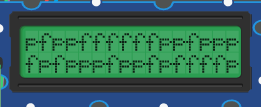
\includegraphics[width=\linewidth]{res/st-pf-04.png}
\end{wrapfigure}

\begin{eleve}	
	\texttt{\textsc{Mission experte 2/3} : Plus de tirages !}
	
	Utiliser les instructions ci-dessous pour effectuer les 32 tirages : 16 sur la première ligne de l'écran et 16 sur la seconde.
	
    \centerline{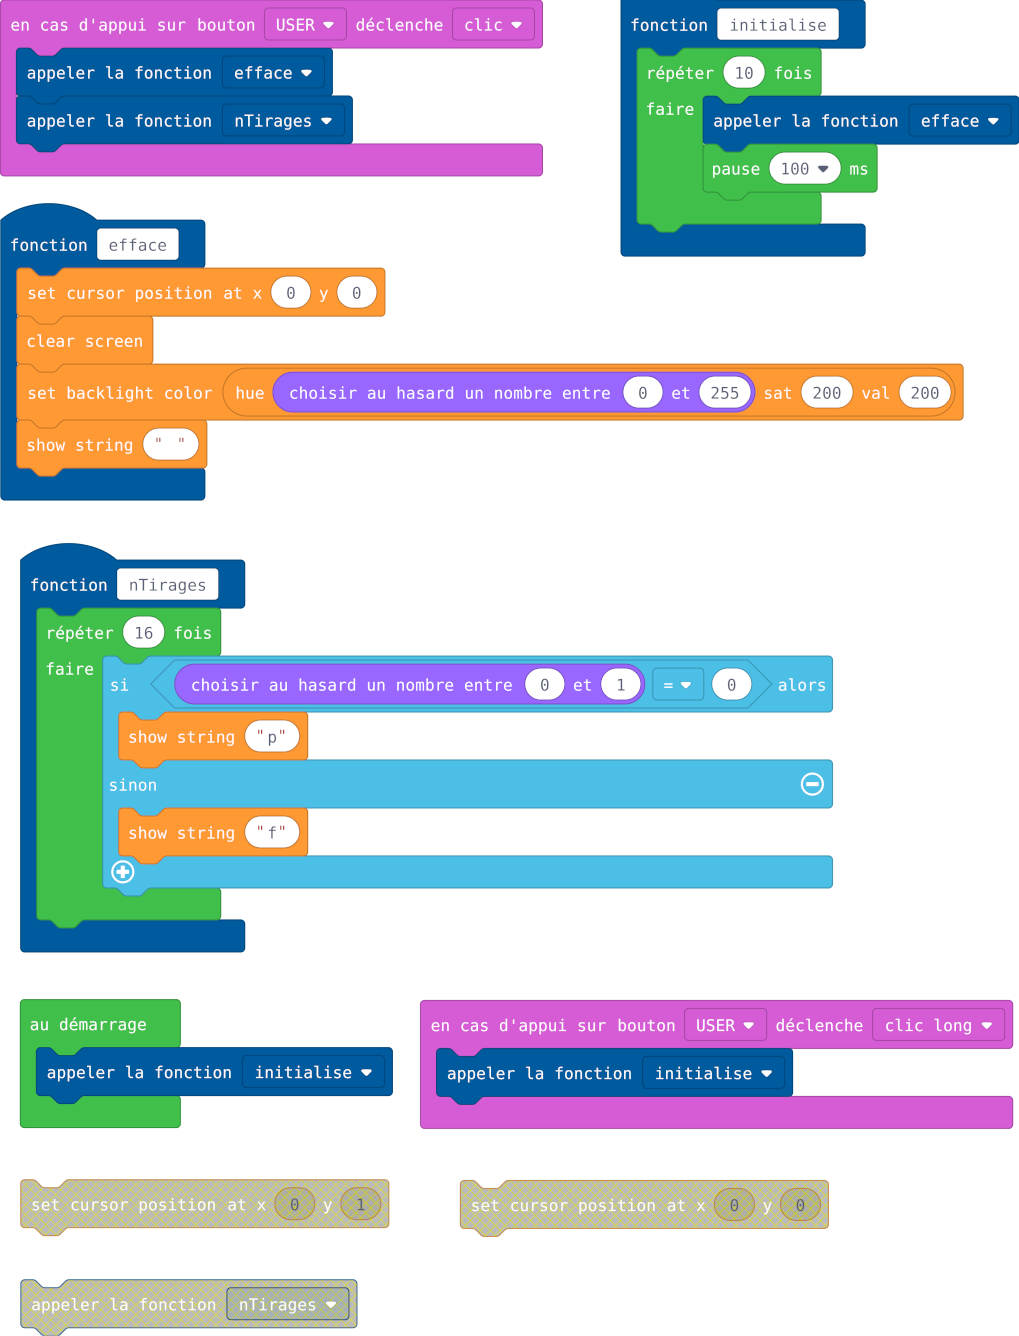
\includegraphics[width=0.6\linewidth]{res/st-pf-04-eleve.png}}
\end{eleve}

\newpage

\begin{minipage}[t]{0.8\linewidth}
    \begin{methode}~\\
        Proposition de résolution :
    
        \centerline{
            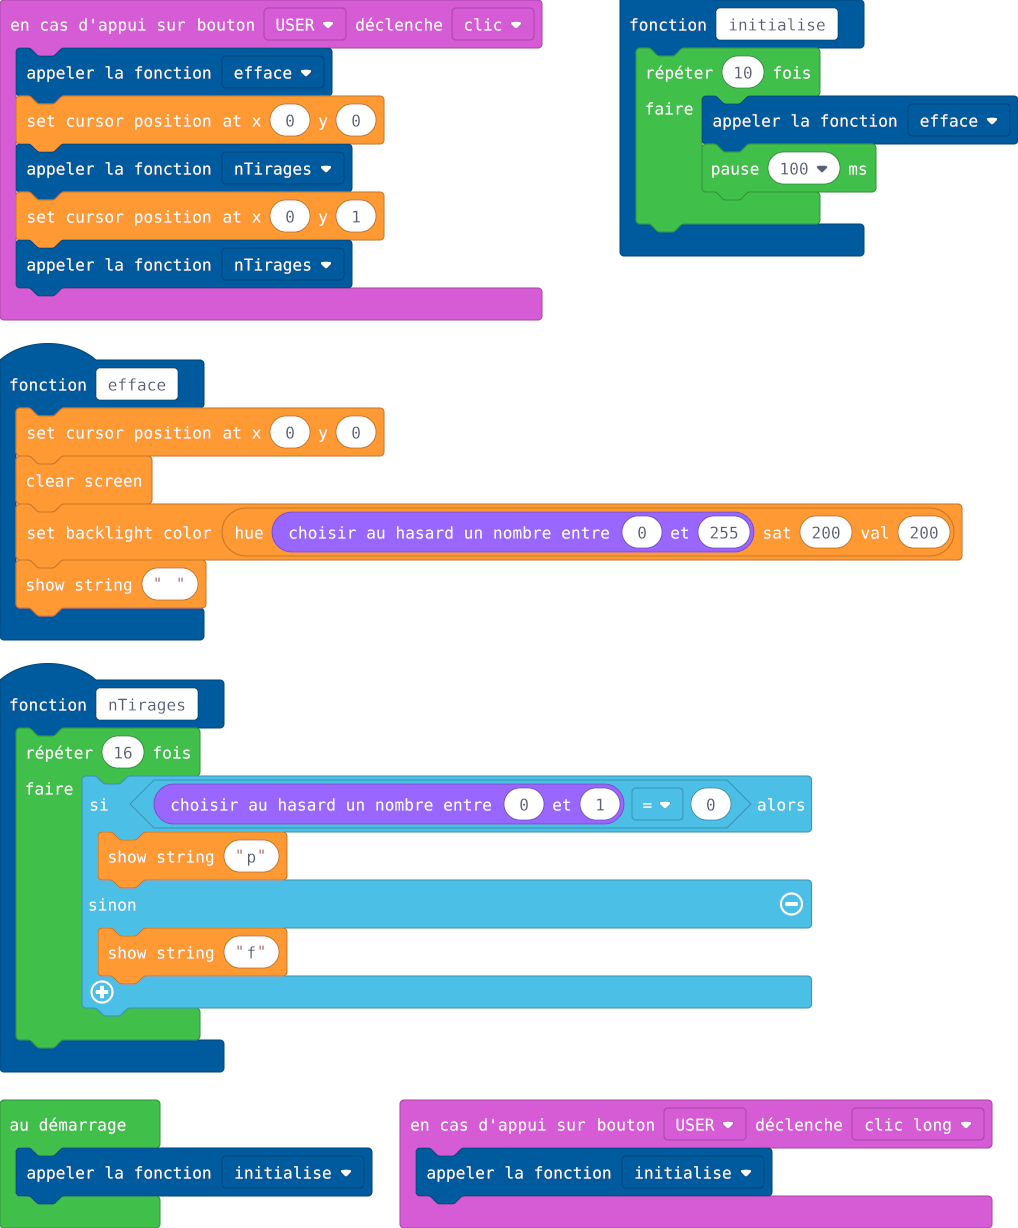
\includegraphics[width=\linewidth]{res/st-pf-04-prof.png}}
\end{methode}
\end{minipage}
\hfill
\begin{minipage}[t]{0.2\linewidth}
    \begin{remarque}~\\
        La proposition de solution \emph{interactive} est accessible en ligne \url{https://makecode.com/_F8MKCVD2jDY8}.
    \end{remarque}
\end{minipage}

%
% activité de niveau 
%
\newpage
\subsection{Niveau expert - Enregistrer les effectifs}
\subsubsection{Activité élève}

% commande perso \CARTOUCHE
%   5 paramètres : 
%       * durée
%       * public
%       * travail en maths
%       * travail en sciences
%       * travail en algo
\cartouche{0,5 h}{2de}{expérience aléatoire}{}{{\footnotesize{affichage ; événement ; fonction ; condition ; boucle ;}} \emph{variables}}


%
%   ELEVE
%


\begin{eleve}
    \begin{minipage}[t]{0.5\linewidth}
        \vspace{0cm}
        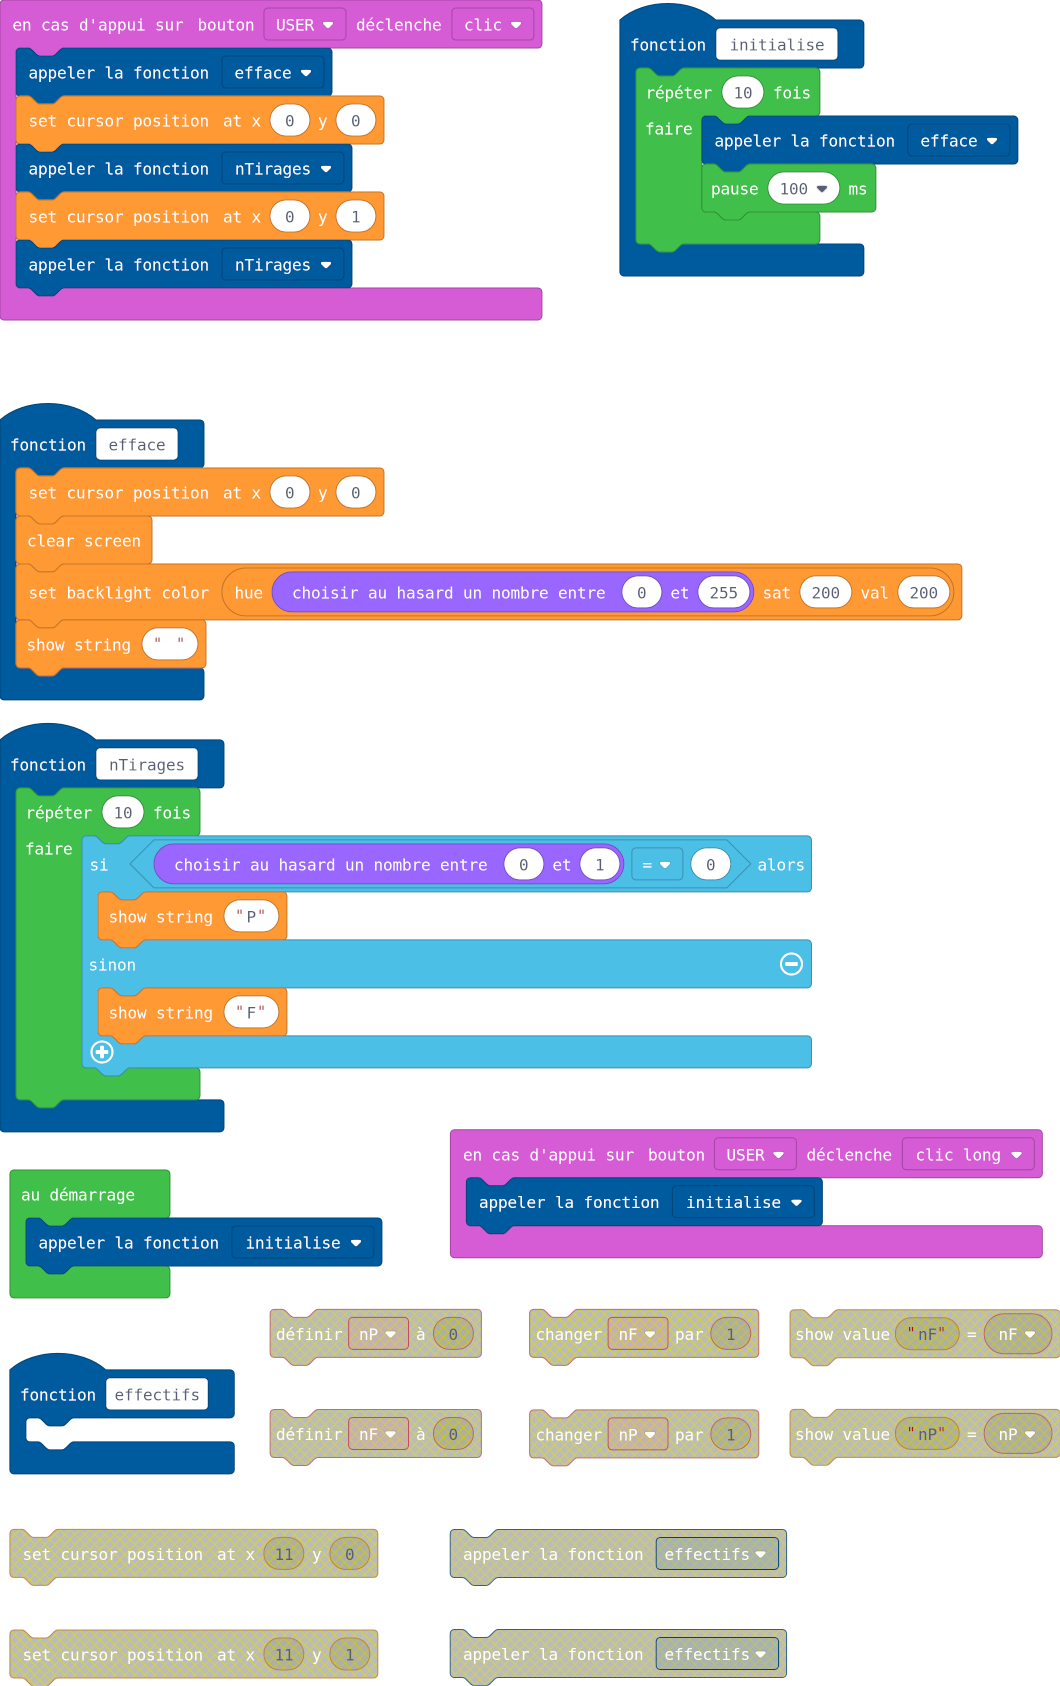
\includegraphics[width=\linewidth]{res/st-pf-05-eleve.png}
    \end{minipage}
    \hfill
    \begin{minipage}[t]{0.4\linewidth}
        \vspace{0cm}
        \hfill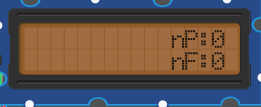
\includegraphics[width=3cm]{res/st-pf-05-1.png}\\
        \hfill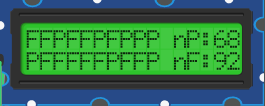
\includegraphics[width=3cm]{res/st-pf-05-2.png}
    
        \texttt{\textsc{Mission experte 3/3} : La totale !}
        
        Pour finir, créer 2 variables \texttt{nP} et \texttt{nF} qui vont compter le nombre total de piles et de faces obtenus. 
        
        Sur chaque ligne, n'effectuer plus que 10 tirages afin de laisser la place pour afficher les valeurs de ces variables.
    \end{minipage}
\end{eleve}

\newpage
\begin{methode}
Proposition de résolution :

\centerline{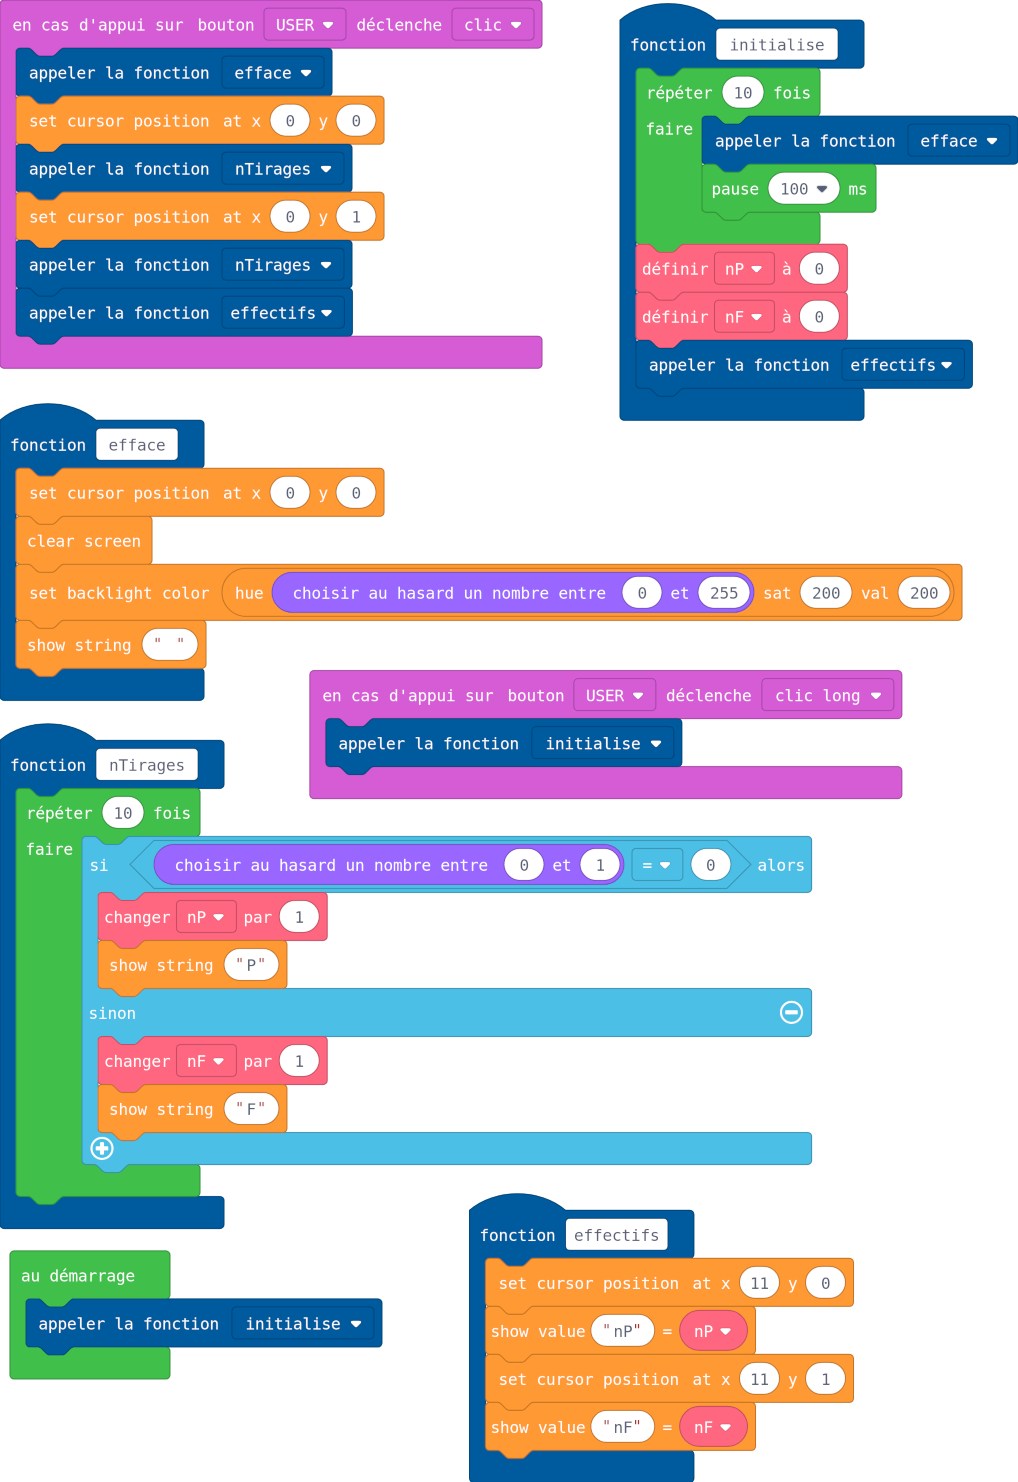
\includegraphics[width=0.75\linewidth]{res/st-pf-05-prof.png}}
\end{methode}

\begin{remarque}
    La proposition de solution \emph{interactive} est accessible en ligne \url{https://makecode.com/_VEy38D1iC07g}.
\end{remarque}
